\newcommand{\Subject}{\textcolor{black}{Thesis Topics Defence}\\{---}\\\LARGE{Warped Hypertime,\\[0.2em] the Tool for Long-Term Autonomy}}
\newcommand{\Meeting}{MESAS 2018, Prague}
\newcommand{\Author}{Tom{\'a}{\v s} Vintr}
%\newcommand{\Authors}{Tom{\'a}{\v s} Vintr, Kerem Eyisoy, Vanda Vintrov{\'a}, Tom{\'a}{\v s} Krajn{\'i}k}
\newcommand{\Authors}{Tom{\'a}{\v s} Vintr}
\newcommand{\Date}{}
%\usetheme{warsaw}

\newcommand{\video}[2]{\href{run:#1}{\includegraphics[width=0.99\textwidth]{#2}}}
\newcommand{\link}[2]{\href{run:#1}{\includegraphics[width=0.99\textwidth]{#2}}}
\newcommand{\bib}[3]{\begin{thebibliography}{#1}\bibitem[#1]{#1}{#2}.\newblock{\em #3}\end{thebibliography}}

\newcommand{\Lincoln}{Artificial Intelligence Center\\Faculty of Electrical Engineering\\Czech Technical University}
\newcommand{\Institute}{\Lincoln\\}


\newcommand{\HeadLineLeft}{Tom{\'a}{\v s} Vintr}
\newcommand{\HeadLineCenter}{Thesis Topics Defence}
\newcommand{\HeadLineRight}{AIC@CTU}
\newcommand{\FootLineCenter}{Warped Hypertime, the Tool for Long-Term Autonomy}
\newcommand{\FootLineLeft}{\insertshortauthor}

% File name: head.tex
% Date:      2008/09/28 20:40
% Author:    Jan Faigl

\newread\testin
\def\softinput #1 {\let\next=\relax \openin\testin=#1
\ifeof\testin \message{Info: the file #1 does not exist}%
\else \closein\testin \def\next{\input #1 }\fi
\next}

\softinput{makeconfig}

\ifx\print\undefined
\documentclass[mathserif]{beamer}
% File name: head-beamer.tex
% Date:      2008/09/28 20:40
% Author:    Jan Faigl

%\usepackage[latin2]{inputenc}
%\usepackage{times}
\usepackage[T1]{fontenc}
\usepackage{helvet}
\usepackage{graphicx}
\usepackage{multimedia}
\usepackage{hyperref}
\usepackage{amsmath}
\usepackage{textcomp}

\usepackage{listings}
\usepackage{ragged2e}

\lstset{extendedchars=true}
\lstset{inputencoding=latin2}
\lstset{breaklines=true,basicstyle=\tiny,language=sh}
\lstset{language=java}
\lstset{columns=fullflexible}
\definecolor{background_color}{gray}{0.9}
\definecolor{comment_color}{rgb}{0.0, 0.5, 0.0}
\definecolor{keyword_color}{rgb}{0.0, 0.0, 1.0}
\definecolor{string_color}{rgb}{0.8, 0.0, 0.0}

\lstset{keywordstyle=\color{keyword_color}\bfseries}
\lstset{commentstyle=\color{comment_color}}
\lstset{stringstyle=\color{string_color}}
\lstset{basicstyle=\ttfamily}
\lstset{showstringspaces=false}
\lstset{keepspaces=true}
\lstset{tabsize=2}
\lstset{breaklines=true}

\institute{\Institute}

\date{\Date}
\author[\Author]{\Authors}
\newcommand{\disable}[1]{}

\colorlet{redshaded}{red!25!bg}
\colorlet{shaded}{black!25!bg}
\colorlet{shadedshaded}{black!10!bg}
\colorlet{blackshaded}{black!40!bg}

\colorlet{darkred}{red!80!black}
\colorlet{darkblue}{blue!80!black}
\colorlet{darkgreen}{green!80!black}

\newcommand{\myurl}[1]{{\color{blue}\url{#1}}}

\DeclareMathOperator{\argmax}{argmax}

\pgfdeclareimage[height=0.4cm]{GL}{fig/gl-logo}
\pgfdeclareimage[height=1.0cm]{logoGL}{fig/logoGL}
%\logo{\pgfuseimage{GL}}
\logo{\pgfuseimage{logoGL}}

\usetheme{Singapore}

\setbeamercovered{transparent}
\setbeamertemplate{navigation symbols}{ }

\defbeamertemplate*{part page}{}[1][]{
\begin{centering}
   {\usebeamerfont{part name}\usebeamercolor[fg]{part name}Part~\insertromanpartnumber}
   \vskip1em\par
   \begin{beamercolorbox}[sep=8pt,center,#1]{part title}
      \usebeamerfont{part title}\insertpart\par
   \end{beamercolorbox}
\end{centering}
}        

\setbeamerfont{code}{size={\fontsize{11pt}{6pt}}}
\setbeamerfont{codeSmall}{size={\fontsize{10pt}{6pt}}}
\setbeamerfont{codeSmaller}{size={\fontsize{9pt}{6pt}}}
\setbeamerfont{small}{size={\fontsize{8pt}{6pt}}}
\AtBeginPart{\frame{\partpage}}


\setbeamercolor{alerted text}{fg=red!80!black}

%-----------------------------------------------------------------------------
% Header line
%-----------------------------------------------------------------------------

\defbeamertemplate*{headline}{}
{%
\begin{beamercolorbox}[colsep=1.5pt]{upper separation line head}
\end{beamercolorbox}
\hbox{%
\begin{beamercolorbox}[wd=0.15\paperwidth,ht=2.25ex,dp=1ex,left]{section in head/foot}%
   \usebeamerfont{title in head/foot}\hspace*{2ex}\HeadLineLeft\hspace*{2ex}
\end{beamercolorbox}%
\begin{beamercolorbox}[wd=0.7\paperwidth,ht=2.25ex,dp=1ex,center]{subsection in head/foot}%
  \usebeamerfont{subsection in head/foot}\hspace*{2ex}\HeadLineCenter
\end{beamercolorbox}%
\begin{beamercolorbox}[wd=0.15\paperwidth,ht=2.25ex,dp=1ex,left]{section in head/foot}%
   \usebeamerfont{section in head/foot}\hspace*{1ex}\HeadLineRight
\end{beamercolorbox}%
}
%\begin{beamercolorbox}{section in head/foot}
%   \vskip2pt\insertsectionnavigationhorizontal{\paperwidth}{}{}\vskip2pt
% \end{beamercolorbox}%

\begin{beamercolorbox}[colsep=1.5pt]{lower separation line head}
\end{beamercolorbox}
}
\addtoheadtemplate{\pgfuseshading{beamer@headfade}\vskip-1.25cm}{}

%-----------------------------------------------------------------------------
% footline
%-----------------------------------------------------------------------------
\defbeamertemplate*{footline}{}{
\leavevmode%
\hbox{%
\begin{beamercolorbox}[wd=.22\paperwidth,ht=2.25ex,dp=1ex,left]{author in head/foot}%
   \usebeamerfont{author in head/foot}\hspace*{2ex}\FootLineLeft\hspace*{2ex}
\end{beamercolorbox}%
\begin{beamercolorbox}[wd=.68\paperwidth,ht=2.25ex,dp=1ex,center]{institute in head/foot}%
   \usebeamerfont{title in head/foot}\FootLineCenter
\end{beamercolorbox}%
\begin{beamercolorbox}[wd=0.1\paperwidth,ht=2.25ex,dp=1ex,right]{date in head/foot}%
   \insertframenumber{} / \inserttotalframenumber\hspace*{1ex}
\end{beamercolorbox}}%
\vskip0pt%
}

\else
\documentclass[trans]{beamer}
% File name: head-print.tex
% Date:      2008/09/28 20:40
% Author:    Jan Faigl

\usepackage[latin2]{inputenc}
\usepackage{times}
\usepackage[T1]{fontenc}
\usepackage{helvet}
\usepackage{graphicx}
\usepackage{multimedia}
\usepackage{hyperref}
\usepackage{amsmath}
\usepackage{textcomp}

\usepackage{listings}
\usepackage{ragged2e}

\lstset{extendedchars=true}
\lstset{inputencoding=latin2}
\lstset{breaklines=true,basicstyle=\tiny,language=sh}
\lstset{language=java}
\lstset{columns=fullflexible}
\definecolor{background_color}{gray}{0.9}
\definecolor{comment_color}{rgb}{0.0, 0.5, 0.0}
\definecolor{keyword_color}{rgb}{0.0, 0.0, 1.0}
\definecolor{string_color}{rgb}{0.8, 0.0, 0.0}

\lstset{keywordstyle=\color{keyword_color}\bfseries}
\lstset{commentstyle=\color{comment_color}}
\lstset{stringstyle=\color{string_color}}
\lstset{basicstyle=\ttfamily}
\lstset{showstringspaces=false}
\lstset{keepspaces=true}
\lstset{tabsize=2}
\lstset{breaklines=true}

\institute{\Institute}

\date{\Date}
\author[\Author]{\Subject}
\newcommand{\disable}[1]{}

\colorlet{redshaded}{red!25!bg}
\colorlet{shaded}{black!25!bg}
\colorlet{shadedshaded}{black!10!bg}
\colorlet{blackshaded}{black!40!bg}

\colorlet{darkred}{red!80!black}
\colorlet{darkblue}{blue!80!black}
\colorlet{darkgreen}{green!80!black}

\newcommand{\myurl}[1]{{\color{blue}\url{#1}}}

\DeclareMathOperator{\argmax}{argmax}

\pgfdeclareimage[height=0.4cm]{GL}{fig/gl-logo}
\pgfdeclareimage[height=0.4cm]{logoGL}{fig/logoGL}
\logo{\pgfuseimage{GL}}
%\logo{\pgfuseimage{logoGL}}

\usetheme{default}

\setbeamercovered{transparent}
\setbeamertemplate{navigation symbols}{ }

\defbeamertemplate*{part page}{}[1][]{
\begin{centering}
   {\usebeamerfont{part name}\usebeamercolor[fg]{part name}��st~\insertromanpartnumber}
   \vskip1em\par
   \begin{beamercolorbox}[sep=8pt,center,#1]{part title}
      \usebeamerfont{part title}\insertpart\par
   \end{beamercolorbox}
\end{centering}
}        

\setbeamerfont{code}{size={\fontsize{11pt}{6pt}}}
\setbeamerfont{codeSmall}{size={\fontsize{10pt}{6pt}}}
\setbeamerfont{codeSmaller}{size={\fontsize{9pt}{6pt}}}
\setbeamerfont{small}{size={\fontsize{8pt}{6pt}}}
\AtBeginPart{\frame{\partpage}}


\setbeamercolor{alerted text}{fg=red!80!black}


%-----------------------------------------------------------------------------
% footline
%-----------------------------------------------------------------------------
\defbeamertemplate*{footlineX}{}{
\leavevmode%
\hbox{%
\begin{beamercolorbox}[wd=.34\paperwidth,ht=2.25ex,dp=1ex,left]{author in head/foot}%
   \usebeamerfont{author in head/foot}\hspace*{2ex}\FootLineLeft\hspace*{2ex}
\end{beamercolorbox}%
\begin{beamercolorbox}[wd=.51\paperwidth,ht=2.25ex,dp=1ex,center]{institute in head/foot}%
   \usebeamerfont{title in head/foot}\FootLineCenter
\end{beamercolorbox}%
\begin{beamercolorbox}[wd=0.14\paperwidth,ht=2.25ex,dp=1ex,right]{date in head/foot}%
   \insertframenumber{} / \inserttotalframenumber\hspace*{1ex}
\end{beamercolorbox}}%
\vskip0pt%
}

\fi


\title{{\bf \Subject}}
\usepackage{multirow}
\begin{document}
% - frame 1---------------------------------------------------------------------

\frame{\titlepage}

\begin{frame}
	\frametitle{SotA in Spatio-temporal Modelling}
    \vspace{3mm}
    \href{run:./video/MorseSpatioTemporalExploration.mp4}{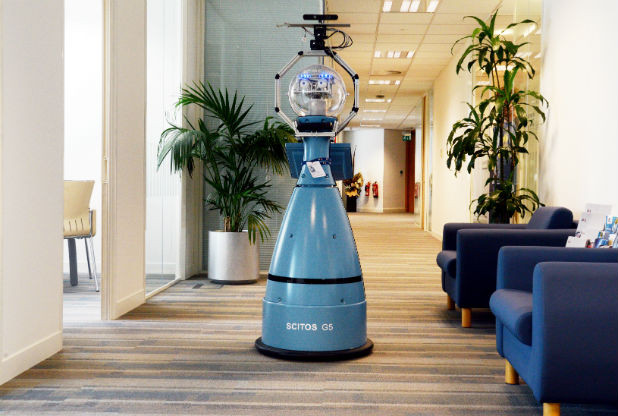
\includegraphics[width=0.9\textwidth]{fig/The-robot-Linda-at-Open-space-office-and-Bob-at-office-corridor.png}}
\end{frame}


% - frame 2---------------------------------------------------------------------

\begin{frame}
	\frametitle{FreMEn - Engine in the Background}
    \vspace{3mm}
    \href{run:./video/pitch.mkv}{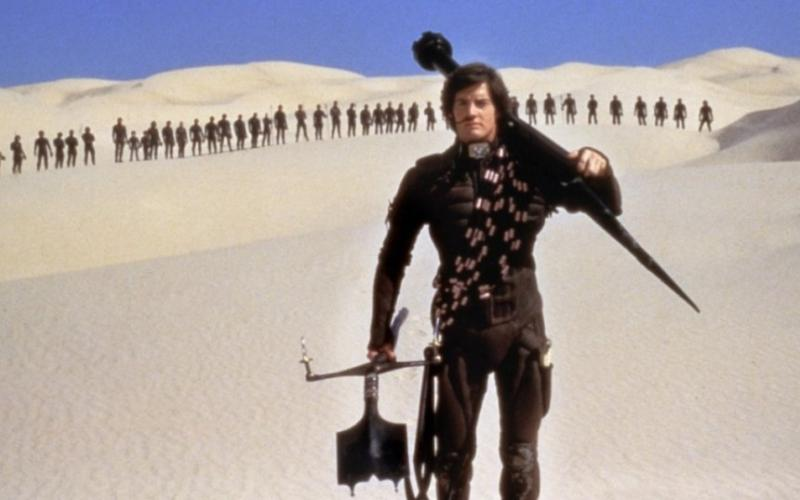
\includegraphics[width=0.9\textwidth]{fig/fremen_backgroung.jpeg}}
\end{frame}


% - frame 3---------------------------------------------------------------------

\begin{frame}
	\frametitle{WHyTe - Projection of Binary Variable}
    \vspace{3mm}
            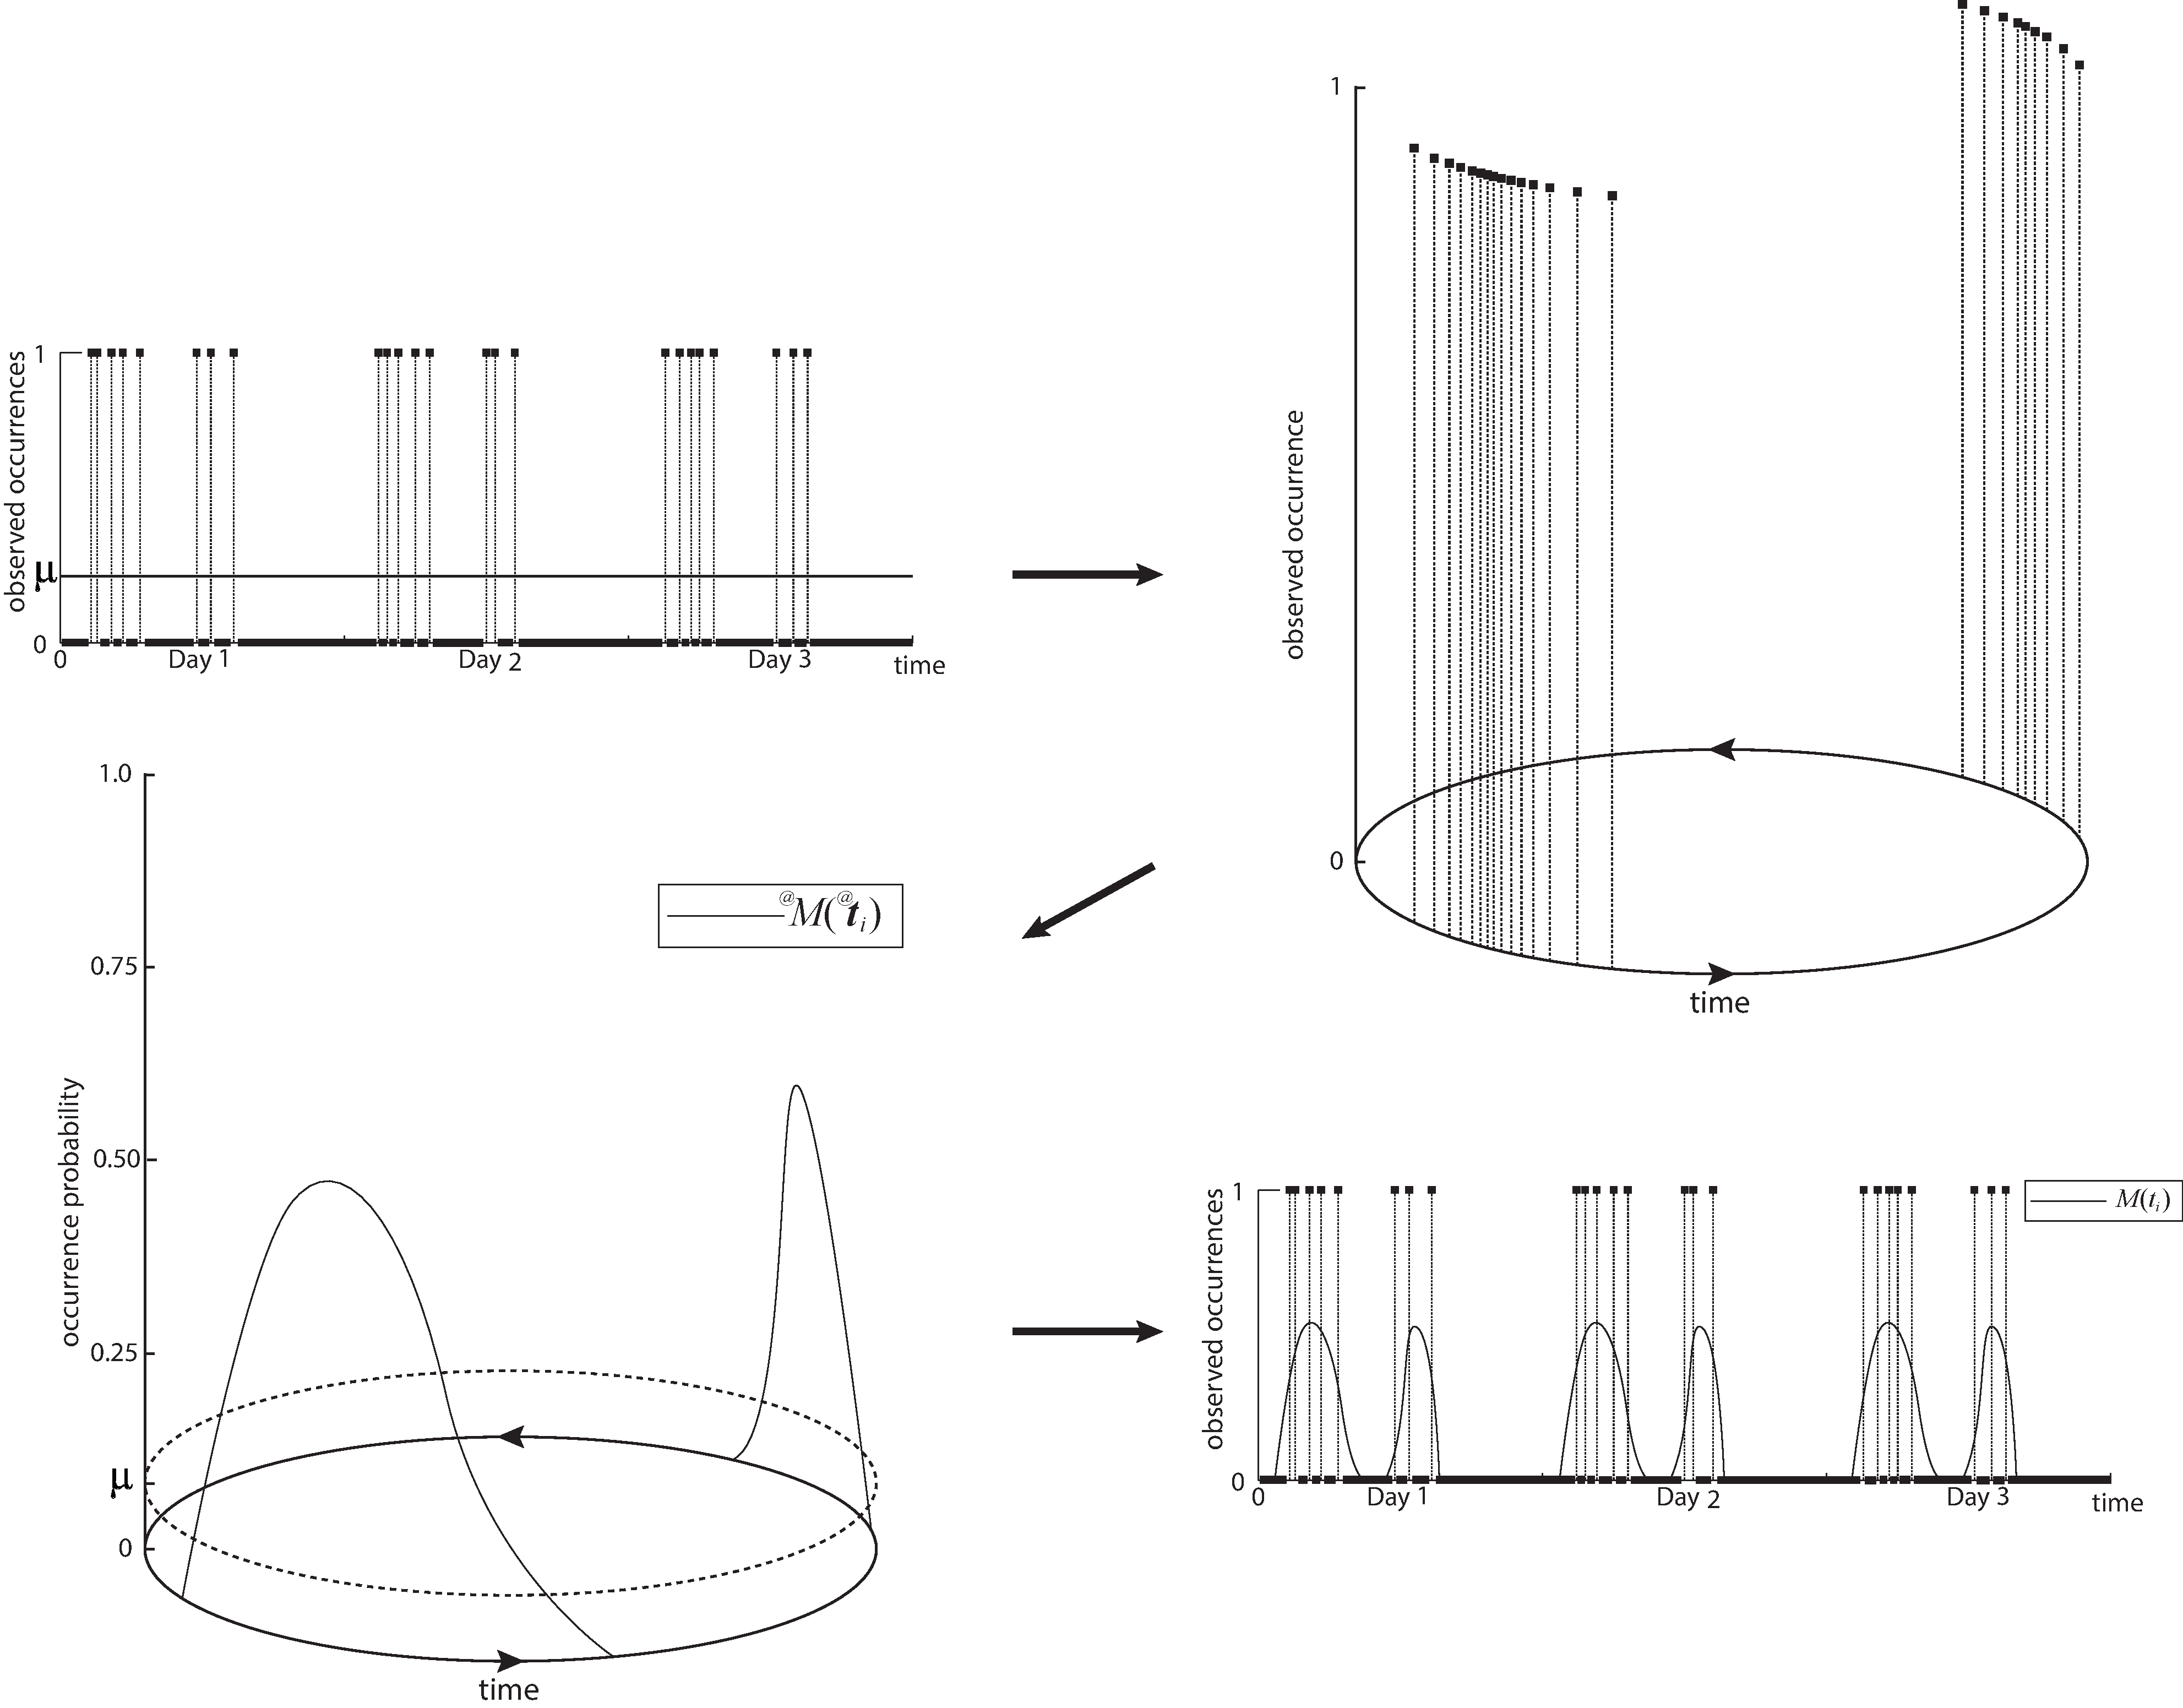
\includegraphics[width=1.0\textwidth]{fig/hypertime_graphs_a.pdf}
\end{frame}


% - frame 4---------------------------------------------------------------------

\begin{frame}
	\frametitle{WHyTeS - Projection of Vector Variable}
    \vspace{3mm}
            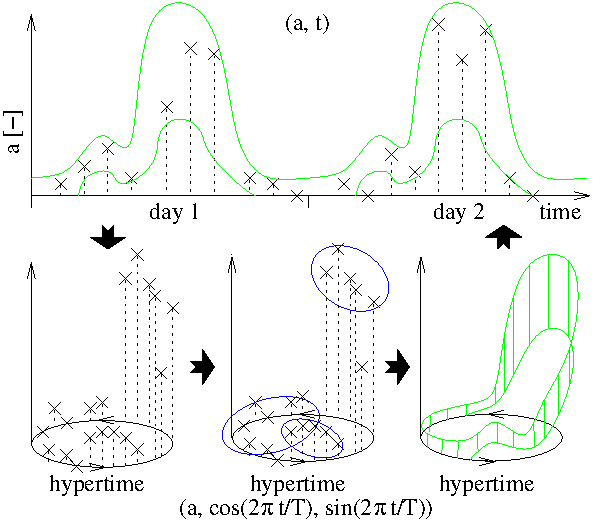
\includegraphics[width=0.8\textwidth]{fig/hypertime_space.pdf}
\end{frame}


% - frame 5---------------------------------------------------------------------

\begin{frame}
	\frametitle{FreMEn Model vs. WHyTe Model}
    \vspace{3mm}
            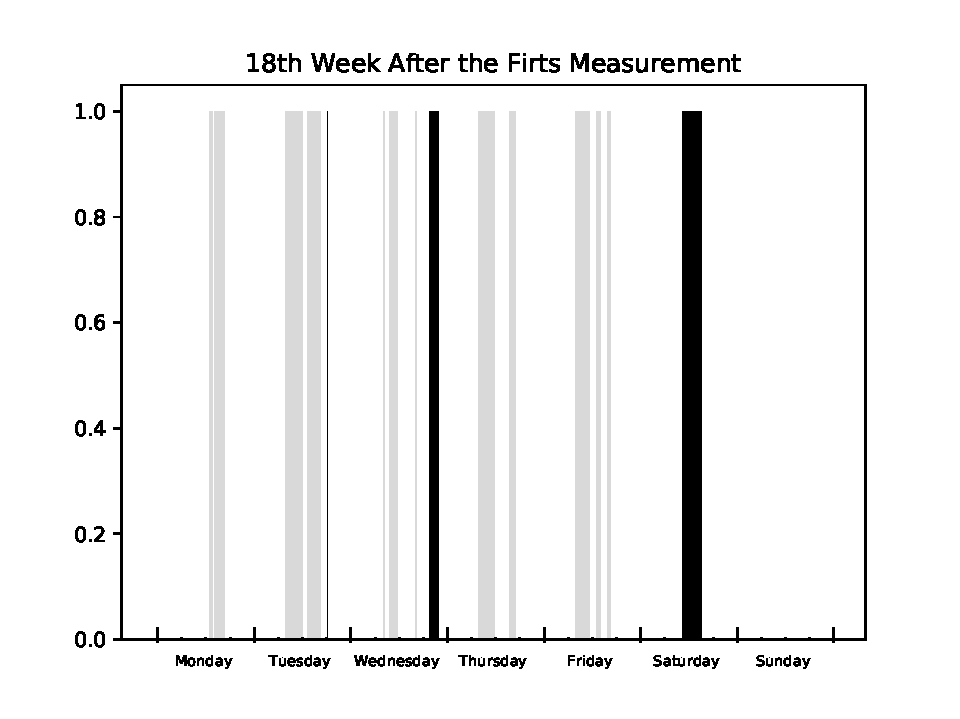
\includegraphics[width=0.8\textwidth]{fig/outliers_test.pdf}
\end{frame}



% - frame 6---------------------------------------------------------------------

\begin{frame}
	\frametitle{Prediction: WHyTe Power $\doteq$ FreMEn Power}
    \vspace{3mm}
\begin{figure}[!b]
   \begin{center}
      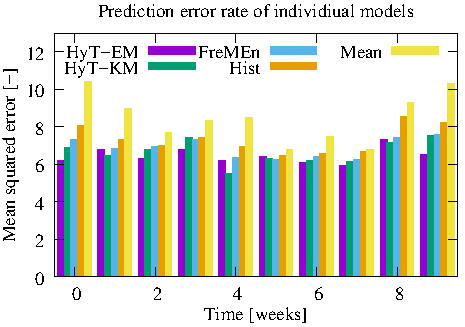
\includegraphics[width=0.45\columnwidth]{fig/door_graph}
    \hfill
      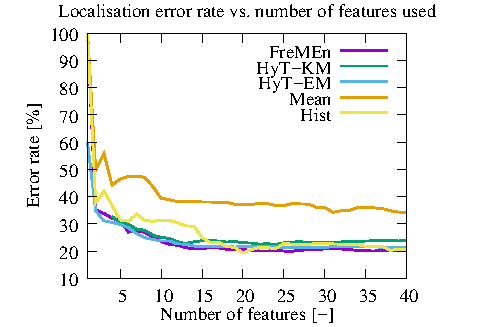
\includegraphics[width=0.45\columnwidth]{fig/localisation_graph}\\\vspace{5mm}
      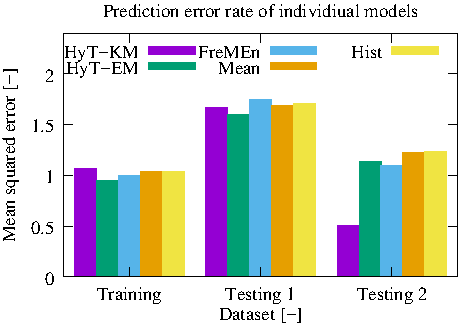
\includegraphics[width=0.45\columnwidth]{fig/nav_graph}
    \hfill
      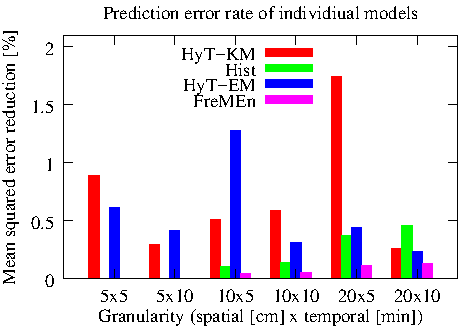
\includegraphics[width=0.45\columnwidth]{fig/ped_graph}
   \end{center}
\end{figure}
\end{frame}


% - frame 7---------------------------------------------------------------------

\begin{frame}
	\frametitle{Memory Efficiency of WHyTeS}
    \vspace{3mm}
\begin{table}[!b]
%\caption{Memory Efficiency of Compared Methods}
\label{tab:ram}
%\resizebox{1.0\textwidth}{!}{%
\centering{
\begin{tabular}{ccccc}
\hline
\begin{tabular}[c]{@{}c@{}}spatial\\cells\end{tabular} & \begin{tabular}[c]{@{}c@{}}WHyTeS\\ c = 3, @ = 2\end{tabular} & \begin{tabular}[c]{@{}c@{}}FreMEn\\ f = 5\end{tabular} & \begin{tabular}[c]{@{}c@{}}Hist\\ h = 24\end{tabular} & Mean      \\ \hline
400                                                          & 1.7 KiB                                                                & 1.1 MiB                                                & 19.3 KiB                                              & 3.3 KiB   \\
1600                                                            & 1.7 KiB                                                                & 4.4 MiB                                                & 307.3 KiB                                             & 12.9 KiB  \\
10000                                                            & 1.7 KiB                                                                & 27.2 MiB                                               & 1.9 MiB                                               & 80.1 KiB  \\
40000                                                            & 1.7 KiB                                                                & 108.9 MiB                                              & 7.7 MiB                                               & 320.1 KiB \\ \hline
\end{tabular}%
}
\end{table}

\end{frame}



% - frame 8---------------------------------------------------------------------

\begin{frame}
	\frametitle{WHyTeS Model Visualisation}
    \vspace{3mm}
    \href{run:./video/WHyTeS_visualisation.mp4}{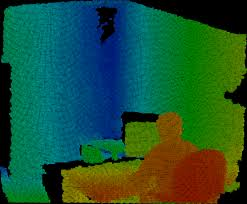
\includegraphics[width=0.7\textwidth]{fig/grzegorz.jpeg}}
\end{frame}



% - frame ---------------------------------------------------------------------
\begin{frame}
	\frametitle{Questions}
	\begin{center}
		%\vfill
		%Code, paper and data available: \textbf{bearnav.eu}
		\vfill
		Thank you for your attention.\\
		\vfill
		Questions?
		\vfill
	\end{center}
\end{frame}


\end{document}
